\documentclass[fleqn,10pt,twocolumn]{wlscirep}
\usepackage[utf8]{inputenc}
\usepackage[T1]{fontenc}
\title{Machine learning number of Dirac cones with neural network}

\author[1]{JunAng Wang}
\author[1,*]{Panagiotis Kotetes}
\affil[1]{CAS Key Laboratory of Theoretical Physics, Institute of Theoretical Physics, Chinese Academy of Sciences, Beijing 100190, China}

\affil[*]{kotetes@mail.itp.ac.cn}

%\affil[+]{these authors contributed equally to this work}

%\keywords{Keyword1, Keyword2, Keyword3}
\twocolumn
\begin{abstract}
Example Abstract. Abstract must not include subheadings or citations. Example Abstract. Abstract must not include subheadings or citations. Example Abstract. Abstract must not include subheadings or citations. Example Abstract. Abstract must not include subheadings or citations. Example Abstract. Abstract must not include subheadings or citations. Example Abstract. Abstract must not include subheadings or citations. Example Abstract. Abstract must not include subheadings or citations. Example Abstract. Abstract must not include subheadings or citations.
\end{abstract}
\begin{document}

\flushbottom
\maketitle
% * <john.hammersley@gmail.com> 2015-02-09T12:07:31.197Z:
%
%  Click the title above to edit the author information and abstract
%
\thispagestyle{empty}

\noindent Please note: Abbreviations should be introduced at the first mention in the main text – no abbreviations lists. Suggested structure of main text (not enforced) is provided below.

\section*{Introduction}

Recent, machine learning has emerged as a powerful tool in various scientific disciplines. Particularly, some researchers have begun to utilize  machine leaning to solve many-body physics problems in the recent year \cite{carleo2019machine,carrasquilla2020machine,johnston2022perspective}, e.g. classifying phases\cite{carrasquilla2017machine,wang2016discovering,tanaka2017detection,zhang2018machine}, representing many-body wave function\cite{carleo2017solving,sharir2020deep}, speeding up many-body simulations\cite{chen2018symmetry,wu2019solving,nagai2017self,liu2017self} et al.   In our previous work titled " Topological Quantization of Superfluid Stiffness in Dirac Materials"\cite{wang2022topological}, we demonstrated the mechanism of the quantization of the superfluid stiffness in Dirac materials. Our findings revealed that the superfluid stiffness in Dirac materials remains quantized as long as the number of Berry monopoles is conserved in the synthetic space. Specifically, in the case of charge-neutral and Zeeman field neutral conditions, the superfluid stiffness($ D_{\textrm{total}}  $) is equal to $  \frac{\Delta}{\pi}  $  per cone (we will derive a more general $ D_{\textrm{total}} $ later ). Therefore the quantity of superfluid stiffness is determined by the number of Dirac cones present. This raises a intriguing question: can we establish a mapping from the value of superfluid stiffness to the number of Dirac cones? Such a mapping would have practical implication allowing experimentalists to determine the number of Dirac cones by measuring the superfluid stiffness of real materials, like graphene.

In this note, we aim to address above question through a supervised machine learning approach. We train our neural network by feeding superfluid stiffness data obtained from the Dirac model that may encompass higher order Dirac cones, enabling it to predict the Hamiltonian's total absolute vorticity. The total absolute vorticity is equal to the number of Dirac cones times their corresponding order.  After fully training our network, we test our model's performance using superfluid stiffness data for graphene which is a 2D material. Our model achieve a high accuracy, which validates the effectiveness of our method.

\section*{Results}


\subsection*{Superfluid stiffness and the total absolute vorticity}

Depict the what is vorticity, why superfluid stiffness embed the information of vorticity (quantized).

\subsection*{Learning vorticity by CNN}

Show the perform accuracy training Dirac model

\subsection*{performance of our neural network testing by graphene}

Network performance testing by graphene

\subsection*{General application of our method}

Training chiral symmetric broken data. Validating by modified graphene.

\section*{Discussion}

The Discussion should be succinct and must not contain subheadings.

\section*{Methods}
\subsection*{Superfluid stiffness computation}
This part discusses the formation of computing superfluid stiffness in Dirac models and graphene model. 


\subsection*{Dataset generation}
Topical subheadings are allowed. Authors must ensure that their Methods section includes adequate experimental and characterization data necessary for others in the field to reproduce their work.

\subsection*{Configuration of our neural network}
This subsection introduce the architecture of our neural network.
\bibliography{refs}

\section*{Acknowledgements (not compulsory)}

Acknowledgements should be brief, and should not include thanks to anonymous referees and editors, or effusive comments. Grant or contribution numbers may be acknowledged.

\section*{Author contributions statement}

Must include all authors, identified by initials, for example:
A.A. conceived the experiment(s),  A.A. and B.A. conducted the experiment(s), C.A. and D.A. analysed the results.  All authors reviewed the manuscript. 

\section*{Additional information}

To include, in this order: \textbf{Accession codes} (where applicable); \textbf{Competing interests} (mandatory statement). 

The corresponding author is responsible for submitting a \href{http://www.nature.com/srep/policies/index.html#competing}{competing interests statement} on behalf of all authors of the paper. This statement must be included in the submitted article file.

\begin{figure}[ht]
\centering
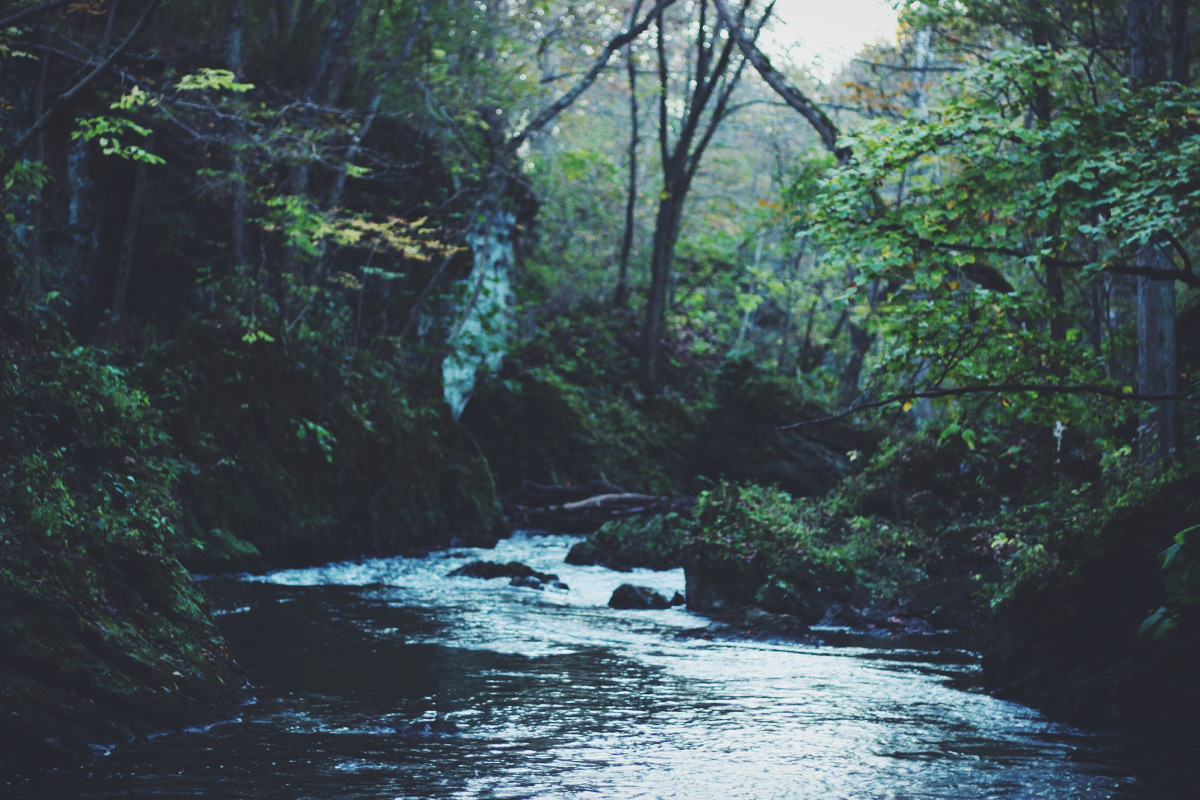
\includegraphics[width=\linewidth]{stream}
\caption{Legend (350 words max). Example legend text.}
\label{fig:stream}
\end{figure}

\begin{table}[ht]
\centering
\begin{tabular}{|l|l|l|}
\hline
Condition & n & p \\
\hline
A & 5 & 0.1 \\
\hline
B & 10 & 0.01 \\
\hline
\end{tabular}
\caption{\label{tab:example}Legend (350 words max). Example legend text.}
\end{table}

Figures and tables can be referenced in LaTeX using the ref command, e.g. Figure \ref{fig:stream} and Table \ref{tab:example}.

\end{document}